\documentclass{article}

\usepackage{ctex}

\usepackage{multicol}

\usepackage[top=1in, bottom=1in, left=1.25in, right=1.25in]{geometry}

\usepackage{lscape}

\usepackage{graphicx}

\usepackage{subfigure}

\author{Shuang Sha}

\date{April 23,2018}

\title{Tech Honcho Wants Innovation for the Bottom Billion\footnote{The source of the article is the Guardian}}




\begin{document}


\maketitle


This paper mainly tells us that a new web standard is expected to kill passwords, meaning users will no longer have to remember difficult logins for each and every website or service they use.

%����ͼƬ
\begin{figure}[htbp]
%\small
\centering
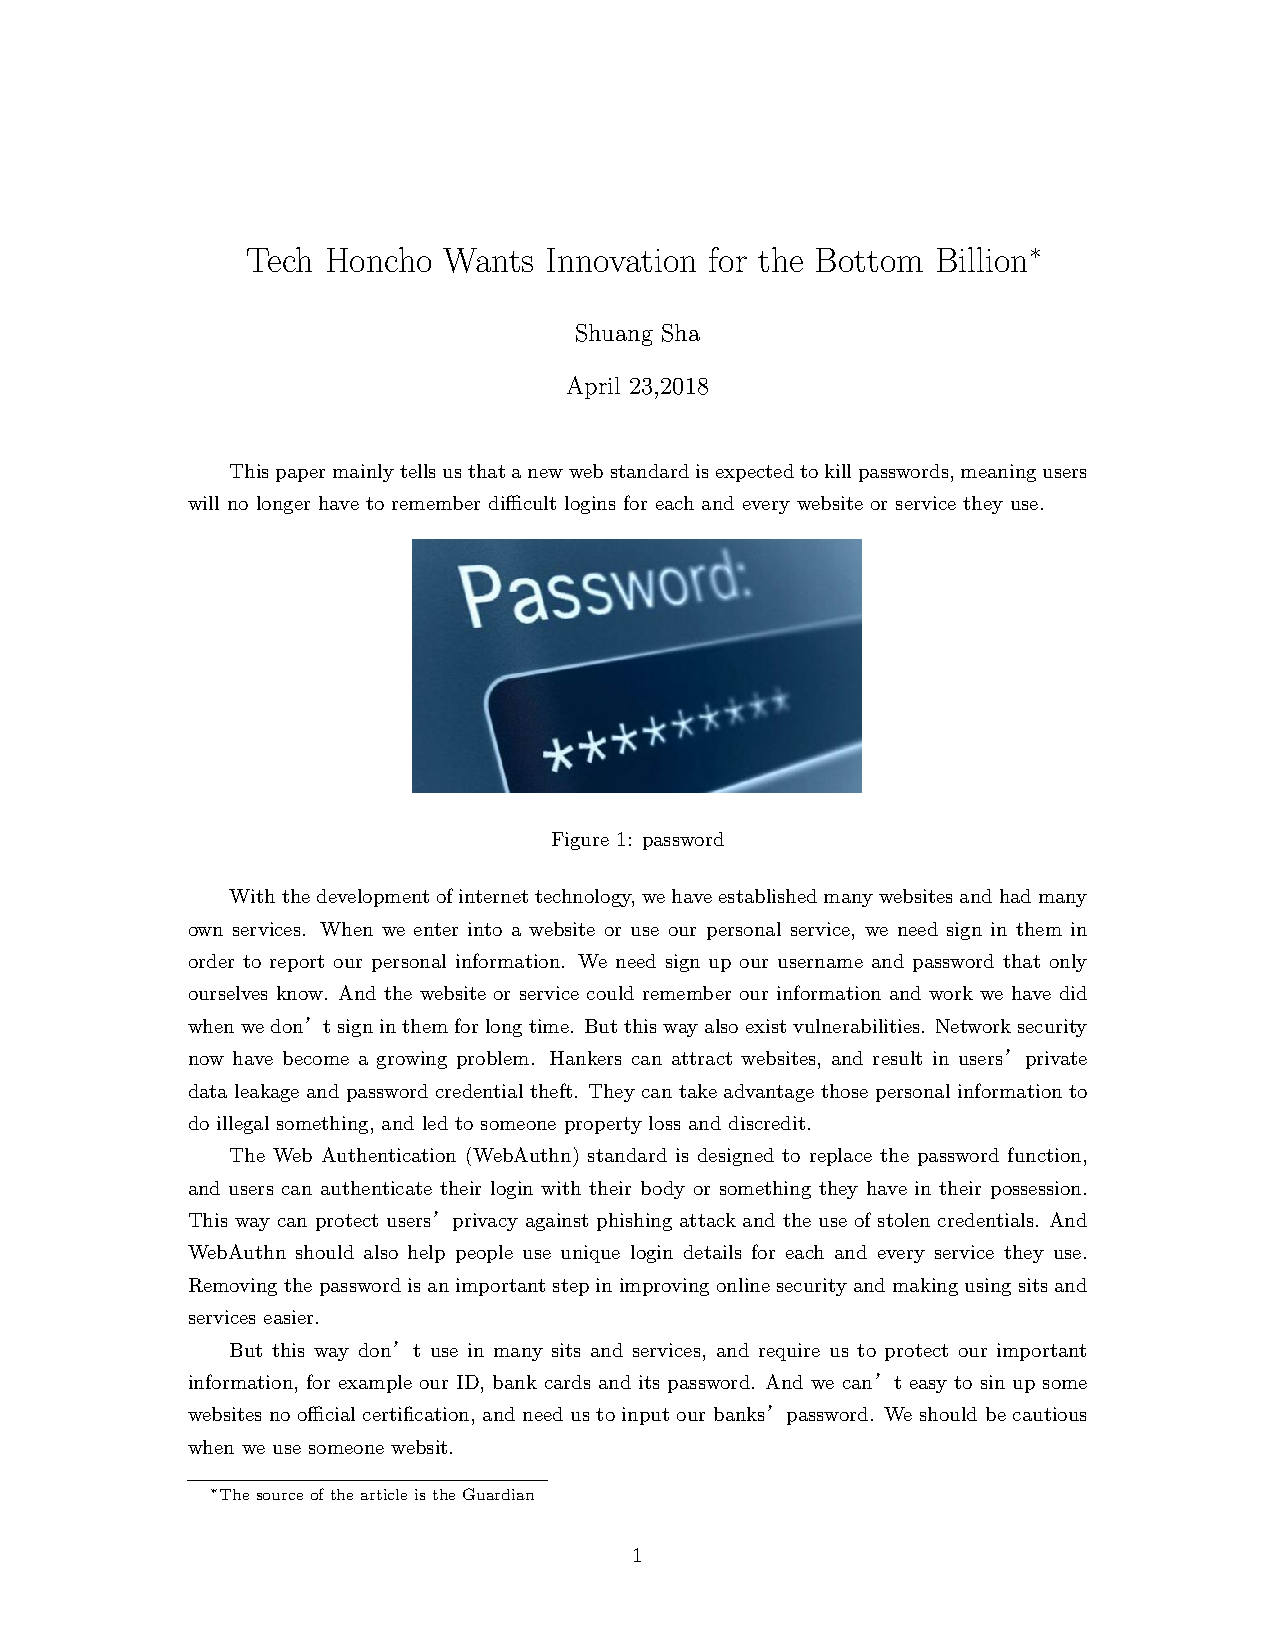
\includegraphics[width=0.5\textwidth]{WebAuthn.jpg}
\caption{password}
   \label{1}
\end{figure}


With the development of internet technology, we have established many websites and had many own services. When we enter into a website or use our personal service, we need sign in them in order to report our personal information. We need sign up our username and password that only ourselves know. And the website or service could remember our information and work we have did when we don��t sign in them for long time. But this way also exist vulnerabilities. Network security now have become a growing problem. Hankers can attract websites, and result in users�� private data leakage and password credential theft. They can take advantage those personal information to do illegal something, and led to someone property loss and discredit.



The Web Authentication (WebAuthn) standard is designed to replace the password function, and users can authenticate their login with their body or something they have in their possession. This way can protect users�� privacy against phishing attack and the use of stolen credentials. And WebAuthn should also help people use unique login details for each and every service they use. Removing the password is an important step in improving online security and making using sits and services easier.



But this way don��t use in many sits and services, and require us to protect our important information, for example our ID, bank cards and its password. And we can��t easy to sin up some websites no official certification, and need us to input our banks�� password. We should be cautious when we use someone websit.




\end{document}

